%\hypertarget{___gatsby}{}
%\hypertarget{gatsby-focus-wrapper}{}
%\href{https://mukulrathi.com/}{}
%
%MUKUL RATHI
%
%\href{https://mukulrathi.com/about-me}{}
%
%About Me
%
%\href{https://mukulrathi.com/blog}{}
%
%Blog
%
%\hypertarget{creating-the-bolt-compiler-part-10}{%
%\subsection{Creating the Bolt Compiler: Part
%10}\label{creating-the-bolt-compiler-part-10}}

\hypertarget{top-of-page}{%
\chapter{Generics - adding polymorphism to Bolt}\label{top-of-page}}

January 23, 2021

%\hypertarget{january-23-2021}{%
%\subsection{January 23, 2021}\label{january-23-2021}}
%
%\hypertarget{min-read}{%
%\subsection{4 min read}\label{min-read}}

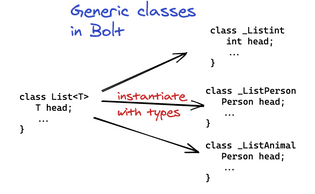
\includegraphics[width=\linewidth]{10_files/generics.png}

%\hypertarget{series-creating-the-bolt-compiler}{%
%\section{Series: Creating the Bolt
%Compiler}\label{series-creating-the-bolt-compiler}}
%
%\begin{itemize}
%\item
%  { Part 1:
%  }\href{https://mukulrathi.com/create-your-own-programming-language/intro-to-compiler/}{How
%  I wrote my own "proper" programming language}
%\item
%  { Part 2:
%  }\href{https://mukulrathi.com/create-your-own-programming-language/compiler-engineering-structure/}{So
%  how do you structure a compiler project?}
%\item
%  { Part 3:
%  }\href{https://mukulrathi.com/create-your-own-programming-language/parsing-ocamllex-menhir/}{Writing
%  a Lexer and Parser using OCamllex and Menhir}
%\item
%  { Part 4:
%  }\href{https://mukulrathi.com/create-your-own-programming-language/intro-to-type-checking/}{An
%  accessible introduction to type theory and implementing a
%  type-checker}
%\item
%  { Part 5:
%  }\href{https://mukulrathi.com/create-your-own-programming-language/data-race-dataflow-analysis/}{A
%  tutorial on liveness and alias dataflow analysis}
%\item
%  { Part 6:
%  }\href{https://mukulrathi.com/create-your-own-programming-language/lower-language-constructs-to-llvm/}{Desugaring
%  - taking our high-level language and simplifying it!}
%\item
%  { Part 7:
%  }\href{https://mukulrathi.com/create-your-own-programming-language/protobuf-ocaml-cpp-tutorial/}{A
%  Protobuf tutorial for OCaml and C++}
%\item
%  { Part 8:
%  }\href{https://mukulrathi.com/create-your-own-programming-language/llvm-ir-cpp-api-tutorial/}{A
%  Complete Guide to LLVM for Programming Language Creators}
%\item
%  { Part 9:
%  }\href{https://mukulrathi.com/create-your-own-programming-language/concurrency-runtime-language-tutorial/}{Implementing
%  Concurrency and our Runtime Library}
%\item
%  \textbf{Part 10: Generics - adding polymorphism to Bolt}
%\item
%  { Part 11:
%  }\href{https://mukulrathi.com/create-your-own-programming-language/inheritance-method-overriding-vtable/}{Adding
%  Inheritance and Method Overriding to Our Language}
%\end{itemize}
%
%\begin{center}\rule{0.5\linewidth}{0.5pt}\end{center}

Onward with more features that any ``proper'' programming language
needs. Today we're implementing \textbf{generics}. Generics allow you to
reuse code for multiple types. Take a \texttt{List} for example. A list
has the same operations regardless of types: it'd be a pain to write out
a new class for each list.

%Copy

\begin{lstlisting}[language=Java]
class ListInt{  ...}
class ListPerson{  ...}
class ListAnimal{  ...}
\end{lstlisting}

The generic class for that would be
\texttt{List\textless{}T\textgreater{}}. We call \texttt{T} the generic
type \emph{parameter}. Think of it like a variable, which we assign a
type to when we instantiate the class:
\texttt{List\textless{}int\textgreater{}()}. Let's build it! We'd like
to compile this program:

%Copy

\begin{lstlisting}[language=Java]
class List<T>{  
    void add(T a){    ...  }  
    T getHead(){    ...  }  
    int size(){    ...  }
}

void main(){  
  let list1 = new List<int>();  
  list1.add(4);  
  ...
}
\end{lstlisting}

\hypertarget{just-give-me-the-code}{%
\section{\texorpdfstring{\protect\hyperlink{just-give-me-the-code}{}Just
give me the
code!}{Just give me the code!}}\label{just-give-me-the-code}}

As ever, the code is in the
\href{https://github.com/mukul-rathi/bolt}{Bolt repo}. The generics are
handled in the
\href{https://github.com/mukul-rathi/bolt/tree/master/src/frontend/typing}{typing}
and
\href{https://github.com/mukul-rathi/bolt/tree/master/src/frontend/desugaring}{desugaring}
stages of the compiler. The code is in the files that contain
\texttt{generics} in their name e.g. \texttt{type\_generics.ml}. You
could even just
\href{https://github.com/mukul-rathi/bolt/search?q=generic}{search
``generic'' in the repo}!

\hypertarget{type-parameters-are-just-like-other-types}{%
\section{\texorpdfstring{\protect\hyperlink{type-parameters-are-just-like-other-types}{}Type
parameters are just like other
types!}{Type parameters are just like other types!}}\label{type-parameters-are-just-like-other-types}}

Rejoice, we don't need to rewrite our type-checker! This tutorial is
much shorter than you think. Here's all that changes in the
type-checker:

\begin{itemize}
\item
  \textbf{Within} our generic class, we can treate our type parameter
  \texttt{T} as an opaque type \texttt{TEGeneric}. So type-check the
  class as before, just don't make any assumptions about \texttt{T}.
\item
  Outside a generic class we can't use generic types \texttt{T}, so
  raise an error if we see that.
\item
  Whenever we use an object instantiated with a type, e.g.
  \texttt{List\textless{}int\textgreater{}}, we can replace all
  occurrences of \texttt{T} with the instantiated type \texttt{int}!
\end{itemize}

That's all that's changed. Seriously!

\hypertarget{treat-the-generic-type-parameter-as-an-opaque-type}{%
\subsection{\texorpdfstring{\protect\hyperlink{treat-the-generic-type-parameter-as-an-opaque-type}{}Treat
the generic type parameter as an opaque
type}{Treat the generic type parameter as an opaque type}}\label{treat-the-generic-type-parameter-as-an-opaque-type}}

We've added to the list of Bolt types a \texttt{TEGeneric} type to
represent this opaque type \texttt{T}.

When we call objects of generic classes, we don't have an object of just
\texttt{List}, it's \texttt{List\textless{}int\textgreater{}},
\texttt{List\textless{}Person\textgreater{}} etc. So we update class
types \texttt{TEClass} to carry around this instantiated type parameter
\texttt{int}, \texttt{Person} etc. if they're generic.
%
%{
%\href{https://github.com/mukul-rathi/bolt/blob/master/src/frontend/ast/ast_types.mli}{ast\_types.ml}}
%
%Copy

\begin{lstlisting}[language=caml,caption={ast\_types.ml}]
type type_expr =  | TEInt  
                 | TEClass   of Class_name.t * type_expr option  
                   (** optionally specify instantiation of type parameter *)  
                 | TEVoid  | TEBool  | TEGeneric
\end{lstlisting}

Next we need to update the \texttt{class\_defn} type to distinguish
between non-generic and generic classes. We define a special type as I
think it's more instructive to see
\texttt{Some\ Generic\ \textbar{}\ None} rather than
\texttt{true\ \textbar{}\ false}. As before, ignore the
\texttt{capability\ list} if you're not interested in the data-race
prevention!
(\href{https://github.com/mukul-rathi/bolt-dissertation/blob/master/dissertation.pdf}{See
my dissertation for a full explanation if you are}).

%{
%\href{https://github.com/mukul-rathi/bolt/blob/master/src/frontend/ast/ast_types.mli}{ast\_types.ml}}
%
%Copy

\begin{lstlisting}[language=caml,caption={ast\_types.ml}]
type generic_type = Generic
\end{lstlisting}

%{
%\href{https://github.com/mukul-rathi/bolt/blob/master/src/frontend/parsing/parsed_ast.ml}{parsed\_ast.ml}}
%
%Copy

\begin{lstlisting}[language=caml,caption={{parsed\_ast.ml}}]
type class_defn = TClass of      Class_name.t      * generic_type option      * capability list (* for data-races (see dissertation) *)      * field_defn list      * method_defn list
\end{lstlisting}

And now, within a generic class \texttt{List}, we instantiate
\texttt{this} to be of type \texttt{List\textless{}T\textgreater{}}
(remember we treat \texttt{T} as an opaque type \texttt{TEGeneric}):
%
%{
%\href{https://github.com/mukul-rathi/bolt/blob/master/src/frontend/typing/type_generics.ml\#L163-L169}{type\_generics.ml}}
%
%Copy

\begin{lstlisting}[language=caml,caption={type\_generics.ml}]
let instantiate_maybe_in_generic_class_this    (Parsed_ast.TClass (class_name, maybe_in_generic_class, _, _, _, _)) =  
   let maybe_type_param =    (* use generic type T inside class *)    
     match maybe_in_generic_class with 
      Some Generic -> Some TEGeneric 
     | None -> None in  (Var_name.of_string "this", TEClass (class_name, maybe_type_param))
\end{lstlisting}

And then the type-checking works as before!

\hypertarget{check-usage-of-generic-types}{%
\subsection{\texorpdfstring{\protect\hyperlink{check-usage-of-generic-types}{}Check
usage of generic
types}{Check usage of generic types}}\label{check-usage-of-generic-types}}

Outside a generic class we can't use generic types. I hate to bore you,
this code is quite mechanical - it's a lot of recursively going through
each of the subexpressions. For a class, check each of the fields,
methods etc. For a function, check its type signature and then its body.
And so on.

Here's a snippet of a function that checks a type. If we're in a generic
class it's all fine, otherwise check we aren't using a generic type.
Click the link to the \texttt{type\_generics.ml} file below to see the
full code.

%{
%\href{https://github.com/mukul-rathi/bolt/blob/master/src/frontend/typing/type_generics.ml\#L5-L21}{type\_generics.ml}}
%
%Copy

\begin{lstlisting}[language=caml,caption={type\_generics.ml}]
let rec type_generics_usage_type type_expr maybe_in_generic_class error_prefix_str =
  match maybe_generic with
  | Some Generic -> Ok () (* can have generics in generic class *)
  | None         -> (    (* recursively check there aren't nested uninitialised type parameters *)
    match type_expr with
    | TEInt | TEBool | TEVoid       -> Ok ()
    | TEGeneric                     ->        Error          (Error.of_string             (Fmt.str "%s Type error: Use of generic type but not in a generic class@."                error_prefix_str))
    | TEClass (_, maybe_type_param) -> (
      match maybe_type_param with
      | Some type_param ->          type_generics_usage_type type_param maybe_in_generic_class error_prefix_str
      | None            -> Ok () ) )
\end{lstlisting}

\hypertarget{instantiate-generic-objects}{%
\subsection{\texorpdfstring{\protect\hyperlink{instantiate-generic-objects}{}Instantiate
generic
objects}{Instantiate generic objects}}\label{instantiate-generic-objects}}

We check first that we should be instantiating with a type-parameter. If
we're trying to instantiate a non-generic class with a type param, raise
an Error, and likewise if we haven't provided a concrete type for a
generic class, raise an error. If we do have a generic class, then
recursively replace all instances of a generic type with the concrete
type: the fields and then the methods etc. Again, full details are in
the repo:

%{
%\href{https://github.com/mukul-rathi/bolt/blob/master/src/frontend/typing/type_generics.ml\#L213-L246}{type\_generics.ml}}
%
%Copy

\begin{lstlisting}[language=caml,caption={type\_generics.ml}]
let instantiate_maybe_generic_class_defn maybe_type_param    ( Parsed_ast.TClass        (class_name, maybe_generic, caps, field_defns, method_defns) as    class_defn ) loc =  
match (maybe_generic, maybe_type_param) with  
  | None, None  (* non-generic class *) ->  Ok class_defn
  | None, Some type_param         ->   Error ...
  | Some Generic, None            -> Error ...
  | Some Generic, Some type_param ->   List.map ~f:(instantiate_maybe_generic_field_defn type_param) field_defns      |> fun instantiated_field_defns ->      List.map ~f:(instantiate_maybe_generic_method_defn type_param) method_defns      |> fun instantiated_method_defns ->      Ok        (Parsed_ast.TClass           ( class_name           , maybe_generic           , caps           , instantiated_field_defns           , instantiated_method_defns ))
\end{lstlisting}

\hypertarget{desugaring-generics}{%
\section{\texorpdfstring{\protect\hyperlink{desugaring-generics}{}Desugaring
Generics}{Desugaring Generics}}\label{desugaring-generics}}

Ok, so we've type-checked our generics, and they pass our checks. What
now? What do we tell our LLVM compiler backend to do when it encounters
a \texttt{T}? You can't allocate a ``generic'' block of memory.

So we \emph{desugar} away all mentions of generic types. What the
compiler backend doesn't know about, it doesn't have to deal with.

Remember, we did this for function overloading
\href{https://mukulrathi.com/create-your-own-programming-language/lower-language-constructs-to-llvm/}{in
our desugaring post}:

%Copy

\begin{verbatim}
function int test(int f) {  ...}
function int test(bool b){  ...}
// DESUGARED (name-mangle functions)
function int testi(int f) {  ...}
function int testb(bool b){  ...}
\end{verbatim}

The compiler backend doesn't need to worry about multiple functions with
the same name, because we handled it in the desugaring stage.

Remember how I said it'd be a pain to write out a new class for each
list? It would be \emph{for us}, as we're doing it by hand. It isn't for
the compiler: it can automate it! To avoid any name-clashes, we'll
prepend each compiler-generated class with an \texttt{\_}.

%Copy

\begin{verbatim}
class _Listint{  ...}
class _ListPerson{  ...}
class _ListAnimal{  ...}
\end{verbatim}

So our desugaring stage has 3 steps to handle generics:

\begin{itemize}
\item
  Count all instantiations of generics
\item
  Create a special class for each of the instantiations (identical to
  how we instantiated generic objects earlier)
\item
  Replace each generic class' constructor with its instantiated class.
  So \texttt{List\textless{}int\textgreater{}} goes to the class
  \texttt{\_Listint}.
\end{itemize}

As before, let's dive into the code!

\hypertarget{count-all-instantiations-of-generics}{%
\subsection{\texorpdfstring{\protect\hyperlink{count-all-instantiations-of-generics}{}Count
all instantiations of
generics}{Count all instantiations of generics}}\label{count-all-instantiations-of-generics}}

This is in the \texttt{count\_generics\_instantiations.ml} file in the
repo (creative name I know!).

We go through the code recursively, and every time we see a constructor
with a concrete type param e.g.
\texttt{List\textless{}int\textgreater{}}, we add that instantiation
\texttt{int} to the total instantiations. In the code below,
\texttt{class\_insts} is a list containing pairs
\texttt{(class\_name,\ list\_of\_types\_instantiated\_with)}:

%{
%\href{https://github.com/mukul-rathi/bolt/blob/master/src/frontend/desugaring/count_generics_instantiations.ml\#L7-L21}{count\_generics\_instantiations.ml}}
%
%Copy

\begin{lstlisting}[language=caml,caption={count\_generics\_instantiations.ml}]
let rec count_generics_instantiations_expr class_defns expr class_insts =  match expr with  | Typed_ast.Constructor (_, class_name, maybe_type_param, constructor_args) ->      ( match maybe_type_param with      | Some TEGeneric  -> class_insts (* only consider concrete type params *)      | Some type_param -> add_instantiation class_defns type_param class_name class_insts      | None            -> class_insts )  ... (* recursive calls *)
\end{lstlisting}

An aside: we can be overly conservative with our counting, as if we
instantiate classes that don't actually get used, then LLVM will
optimise them away. So we could have brute-forced all possible
combinations - this would have slowed the compiler down, but it wouldn't
have affected the code output.

\hypertarget{replace-generic-classes-with-instantiated-classes}{%
\subsection{\texorpdfstring{\protect\hyperlink{replace-generic-classes-with-instantiated-classes}{}Replace
generic classes with instantiated
classes}{Replace generic classes with instantiated classes}}\label{replace-generic-classes-with-instantiated-classes}}

The first step is to replace the class definitions: below we instantiate
all the generic classes with concrete types, then filter the original
generic classes out and return the updated list of classes.

%{
%\href{https://github.com/mukul-rathi/bolt/blob/master/src/frontend/desugaring/replace_generic_with_instantiated_class_defns.ml\#L195-L210}{replace\_generic\_with\_instantiated\_class\_defns.ml}}
%
%Copy

\begin{lstlisting}[caption={replace\_generic\_with\_instantiated\_class\_defns.ml},language=caml]
let replace_generic_with_instantiated_class_defns class_defns class_insts =  List.map    ~f:(fun (class_name, type_params) ->      List.find_exn        ~f:(fun (Typed_ast.TClass (name, _, _, _, _, _)) -> name = class_name)        class_defns      |> fun class_defn -> instantiate_generic_class_defn type_params class_defn)    class_insts  |> fun instantiated_class_defns ->  (* get rid of uninitialised generic classes *)  List.filter    ~f:(fun (Typed_ast.TClass (_, maybe_generic, _, _, _, _)) ->      match maybe_generic with Some Generic -> false | None -> true)    class_defns  |> fun non_generic_class_defns ->  List.concat (non_generic_class_defns :: instantiated_class_defns)
\end{lstlisting}

We then need to replace all references to generic classes in the program
with the special instances (we name-mangle them). Inside the compiler we
convert \texttt{List\textless{}int\textgreater{}} to \texttt{\_Listint}.
Again, the code is mechanical and a lot of recursive cases replacing
generic class names with the new instantiated class:

%{
%\href{https://github.com/mukul-rathi/bolt/blob/master/src/frontend/desugaring/name_mangle_generics.ml\#L5-7}{name\_mangle\_generics.ml}}
%
%Copy

\begin{lstlisting}[language=caml,caption={name\_mangle\_generics.ml}]
let name_mangle_generic_class class_name type_param =  Class_name.of_string    (Fmt.str "_%s%s" (Class_name.to_string class_name) (string_of_type type_param))
\end{lstlisting}

\hypertarget{summary}{%
\section{\texorpdfstring{\protect\hyperlink{summary}{}Summary}{Summary}}\label{summary}}

That's it! We only had to modify our type-checker and desugaring stage
to handle generics, and most of the code was just going through each
sub-expression recursively.

This approach of replacing a generic class with specialised instances
(one for each concrete type) is called \textbf{monomorphism} and it is
what C++ does with its templates. If you want to find out more about how
other languages implement generics,
\href{https://www.thomasdenney.co.uk/blog/2016/11/13/comparing-the-implementation-of-generics/}{check
out this blog post} for a more technical read.

%\hypertarget{share-this-on-twitter}{%
%\subsection{Share This On Twitter}\label{share-this-on-twitter}}
%
%If you liked this post, please consider sharing it with your network. If
%you have any questions, tweet away and I'll answer :) I also tweet when
%new posts drop!
%
%\textbf{PS:} I also share helpful tips and links as I'm learning - so
%you get them \textbf{well before} they make their way into a post!
%
%\hypertarget{series-creating-the-bolt-compiler-1}{%
%\section{Series: Creating the Bolt
%Compiler}\label{series-creating-the-bolt-compiler-1}}
%
%\begin{itemize}
%\item
%  { Part 1:
%  }\href{https://mukulrathi.com/create-your-own-programming-language/intro-to-compiler/}{How
%  I wrote my own "proper" programming language}
%\item
%  { Part 2:
%  }\href{https://mukulrathi.com/create-your-own-programming-language/compiler-engineering-structure/}{So
%  how do you structure a compiler project?}
%\item
%  { Part 3:
%  }\href{https://mukulrathi.com/create-your-own-programming-language/parsing-ocamllex-menhir/}{Writing
%  a Lexer and Parser using OCamllex and Menhir}
%\item
%  { Part 4:
%  }\href{https://mukulrathi.com/create-your-own-programming-language/intro-to-type-checking/}{An
%  accessible introduction to type theory and implementing a
%  type-checker}
%\item
%  { Part 5:
%  }\href{https://mukulrathi.com/create-your-own-programming-language/data-race-dataflow-analysis/}{A
%  tutorial on liveness and alias dataflow analysis}
%\item
%  { Part 6:
%  }\href{https://mukulrathi.com/create-your-own-programming-language/lower-language-constructs-to-llvm/}{Desugaring
%  - taking our high-level language and simplifying it!}
%\item
%  { Part 7:
%  }\href{https://mukulrathi.com/create-your-own-programming-language/protobuf-ocaml-cpp-tutorial/}{A
%  Protobuf tutorial for OCaml and C++}
%\item
%  { Part 8:
%  }\href{https://mukulrathi.com/create-your-own-programming-language/llvm-ir-cpp-api-tutorial/}{A
%  Complete Guide to LLVM for Programming Language Creators}
%\item
%  { Part 9:
%  }\href{https://mukulrathi.com/create-your-own-programming-language/concurrency-runtime-language-tutorial/}{Implementing
%  Concurrency and our Runtime Library}
%\item
%  \textbf{Part 10: Generics - adding polymorphism to Bolt}
%\item
%  { Part 11:
%  }\href{https://mukulrathi.com/create-your-own-programming-language/inheritance-method-overriding-vtable/}{Adding
%  Inheritance and Method Overriding to Our Language}
%\end{itemize}
%
%\begin{itemize}
%\item ~
%  \hypertarget{write-it-and-they-will-eventually-come}{%
%  \subsection{\texorpdfstring{\href{https://mukulrathi.com/2020-blog-review/}{←
%  Write It and They Will (Eventually)
%  Come}}{← Write It and They Will (Eventually) Come}}\label{write-it-and-they-will-eventually-come}}
%\item ~
%  \hypertarget{adding-inheritance-and-method-overriding-to-our-language}{%
%  \subsection{\texorpdfstring{\href{https://mukulrathi.com/create-your-own-programming-language/inheritance-method-overriding-vtable/}{Adding
%  Inheritance and Method Overriding to Our Language
%  →}}{Adding Inheritance and Method Overriding to Our Language →}}\label{adding-inheritance-and-method-overriding-to-our-language}}
%\end{itemize}
%
%\hypertarget{table-of-contents}{%
%\section{Table of Contents}\label{table-of-contents}}
%
%\href{https://mukulrathi.com/create-your-own-programming-language/generics-parametric-polymorphism/\#top-of-page}{}
%
%\hypertarget{generics---adding-polymorphism-to-bolt}{%
%\subsection{Generics - adding polymorphism to
%Bolt}\label{generics---adding-polymorphism-to-bolt}}
%
%\begin{itemize}
%\item
%  \href{https://mukulrathi.com/create-your-own-programming-language/generics-parametric-polymorphism/\#just-give-me-the-code}{}
%
%  \hypertarget{just-give-me-the-code-1}{%
%  \subsection{Just give me the code!}\label{just-give-me-the-code-1}}
%\item
%  \href{https://mukulrathi.com/create-your-own-programming-language/generics-parametric-polymorphism/\#type-parameters-are-just-like-other-types}{}
%
%  \hypertarget{type-parameters-are-just-like-other-types-1}{%
%  \subsection{Type parameters are just like other
%  types!}\label{type-parameters-are-just-like-other-types-1}}
%
%  \begin{itemize}
%  \item
%    \href{https://mukulrathi.com/create-your-own-programming-language/generics-parametric-polymorphism/\#treat-the-generic-type-parameter-as-an-opaque-type}{}
%
%    \hypertarget{treat-the-generic-type-parameter-as-an-opaque-type-1}{%
%    \subsection{Treat the generic type parameter as an opaque
%    type}\label{treat-the-generic-type-parameter-as-an-opaque-type-1}}
%  \item
%    \href{https://mukulrathi.com/create-your-own-programming-language/generics-parametric-polymorphism/\#check-usage-of-generic-types}{}
%
%    \hypertarget{check-usage-of-generic-types-1}{%
%    \subsection{Check usage of generic
%    types}\label{check-usage-of-generic-types-1}}
%  \item
%    \href{https://mukulrathi.com/create-your-own-programming-language/generics-parametric-polymorphism/\#instantiate-generic-objects}{}
%
%    \hypertarget{instantiate-generic-objects-1}{%
%    \subsection{Instantiate generic
%    objects}\label{instantiate-generic-objects-1}}
%  \end{itemize}
%\item
%  \href{https://mukulrathi.com/create-your-own-programming-language/generics-parametric-polymorphism/\#desugaring-generics}{}
%
%  \hypertarget{desugaring-generics-1}{%
%  \subsection{Desugaring Generics}\label{desugaring-generics-1}}
%
%  \begin{itemize}
%  \item
%    \href{https://mukulrathi.com/create-your-own-programming-language/generics-parametric-polymorphism/\#count-all-instantiations-of-generics}{}
%
%    \hypertarget{count-all-instantiations-of-generics-1}{%
%    \subsection{Count all instantiations of
%    generics}\label{count-all-instantiations-of-generics-1}}
%  \item
%    \href{https://mukulrathi.com/create-your-own-programming-language/generics-parametric-polymorphism/\#replace-generic-classes-with-instantiated-classes}{}
%
%    \hypertarget{replace-generic-classes-with-instantiated-classes-1}{%
%    \subsection{Replace generic classes with instantiated
%    classes}\label{replace-generic-classes-with-instantiated-classes-1}}
%  \end{itemize}
%\item
%  \href{https://mukulrathi.com/create-your-own-programming-language/generics-parametric-polymorphism/\#summary}{}
%
%  \hypertarget{summary-1}{%
%  \subsection{Summary}\label{summary-1}}
%\end{itemize}
%
%© Mukul Rathi 2023
%
%\hypertarget{gatsby-announcer}{}
%Navigated to Generics - adding polymorphism to Bolt
